\section{Risultati della sperimentazione}
Si presentano ora i risultati quantitativi della sperimentazione effettuata sui
cinque pannelli scelti tra quelli ottenuti nella \textit{phase 3} del
\textit{1000 Genome Project}. Come anticipato, al fine del computo degli SMEM,
avendo un numero 
ridotto di sample a disposizione, si è scelto di estrarre da ognuno 100 sample
da usare come query, riducendo quindi il numero di sample a 4.908.
\subsection{Costruzione delle strutture e calcolo degli SMEM}
Viste le dimensioni di tali pannelli si ritiene necessario studiare, dal punto
di vista del tempo macchina e dei picchi di memoria necessaria, le varie fasi
della sperimentazione, ovvero:
\begin{itemize}
  \item la fase di \textit{preprocessing}, necessaria per la preparazione dei
  vari input della\textit{RLPBWT}, comprendente: 
  \begin{itemize}
    \item la conversione dei file in formato VCF nei file in formato MACs
    \item l'estrazione del pannello delle query e la creazione del nuovo
    pannello di aplotipi reference
    \item la produzione dell\textit{SLP} del pannello di reference, comprendente
    sia la produzione della stringa unica monodimensionale che l'esecuzione di
    \textit{BigRepair} e \textit{ShapedSlp}
  \end{itemize}
  \item la costruzione e serializzazione delle varie strutture dati composte per
  la \textit{RLPBWT} e dei file ad hoc per la \textit{PBWT}
  \item il calcolo degli \textit{SMEM}
\end{itemize}
\paragraph{Preprocessing.}
In figura \ref{fig:prechr} si possono analizzare le prestazioni delle tre
fasi di preprocessing. I risultati quantitativi sono consultabili alla tabella
\ref{tab:prepmem} e alla tabella \ref{tab:preptime}. La separazione del
pannello con le query risulta essere assolutamente 
ininfluente e, di fatto, anche la conversione tra i due formati non
necessita particolari considerazioni, come inferibile dai risultati numerici
delle performance. Tale conversione 
diventerebbe non necessaria implementando l'input direttamente da file VCF per
le varie strutture dati relative alla \textit{RLPBWT}. Inoltre, in un contesto
reale, la costruzione del pannello di query non sarebbe un'operazione
necessaria.\\
Bisogna, però, analizzare la costruzione 
dell'\textit{SLP}. Per quanto quest'operazione sia da svolgersi \textit{una
  tantum}, le richieste in termini di memoria sono nell'ordine delle centinaia
di gigabytes di RAM mentre i tempi di calcolo sono nell'ordine delle
ore. Prendendo in analisi il cromosoma 1 si ha infatti che è richiesto un picco
di 644GB di RAM, avendo che l'intera esecuzione richiede circa 4 ore.
D'altro canto, bisogna considerare che tutti gli strumenti computazionali per la
produzione 
dell'\textit{SLP} sono studiati per partire da una singola stringa e non da una
matrice. Nuovi sviluppi in questa direzione potrebbero lasciar spazio a diverse
ottimizzazioni. Bisogna, infine, considerare che
questa fase è necessaria solo per quattro delle sei soluzioni studiate per la
\textit{RLPBWT} basate sul calcolo delle \textit{matching statistics} e, come
già detto, il fatto che sia necessaria solo una volta 
è cruciale nell'ottica di un confronto con, ad esempio,
lo spazio richiesto dall'\textit{algoritmo 5} di Durbin, che richiede $13NM$
bytes per il calcolo degli \textit{SMEM} ad ogni esecuzione.\\
In generale, la crescita di memoria richiesta e di tempi per le tre fasi di
preprocessing sembrano essere proporzionali al numero di siti dei pannelli, come
ci si potrebbe attendere.
\begin{figure}
  \centering
  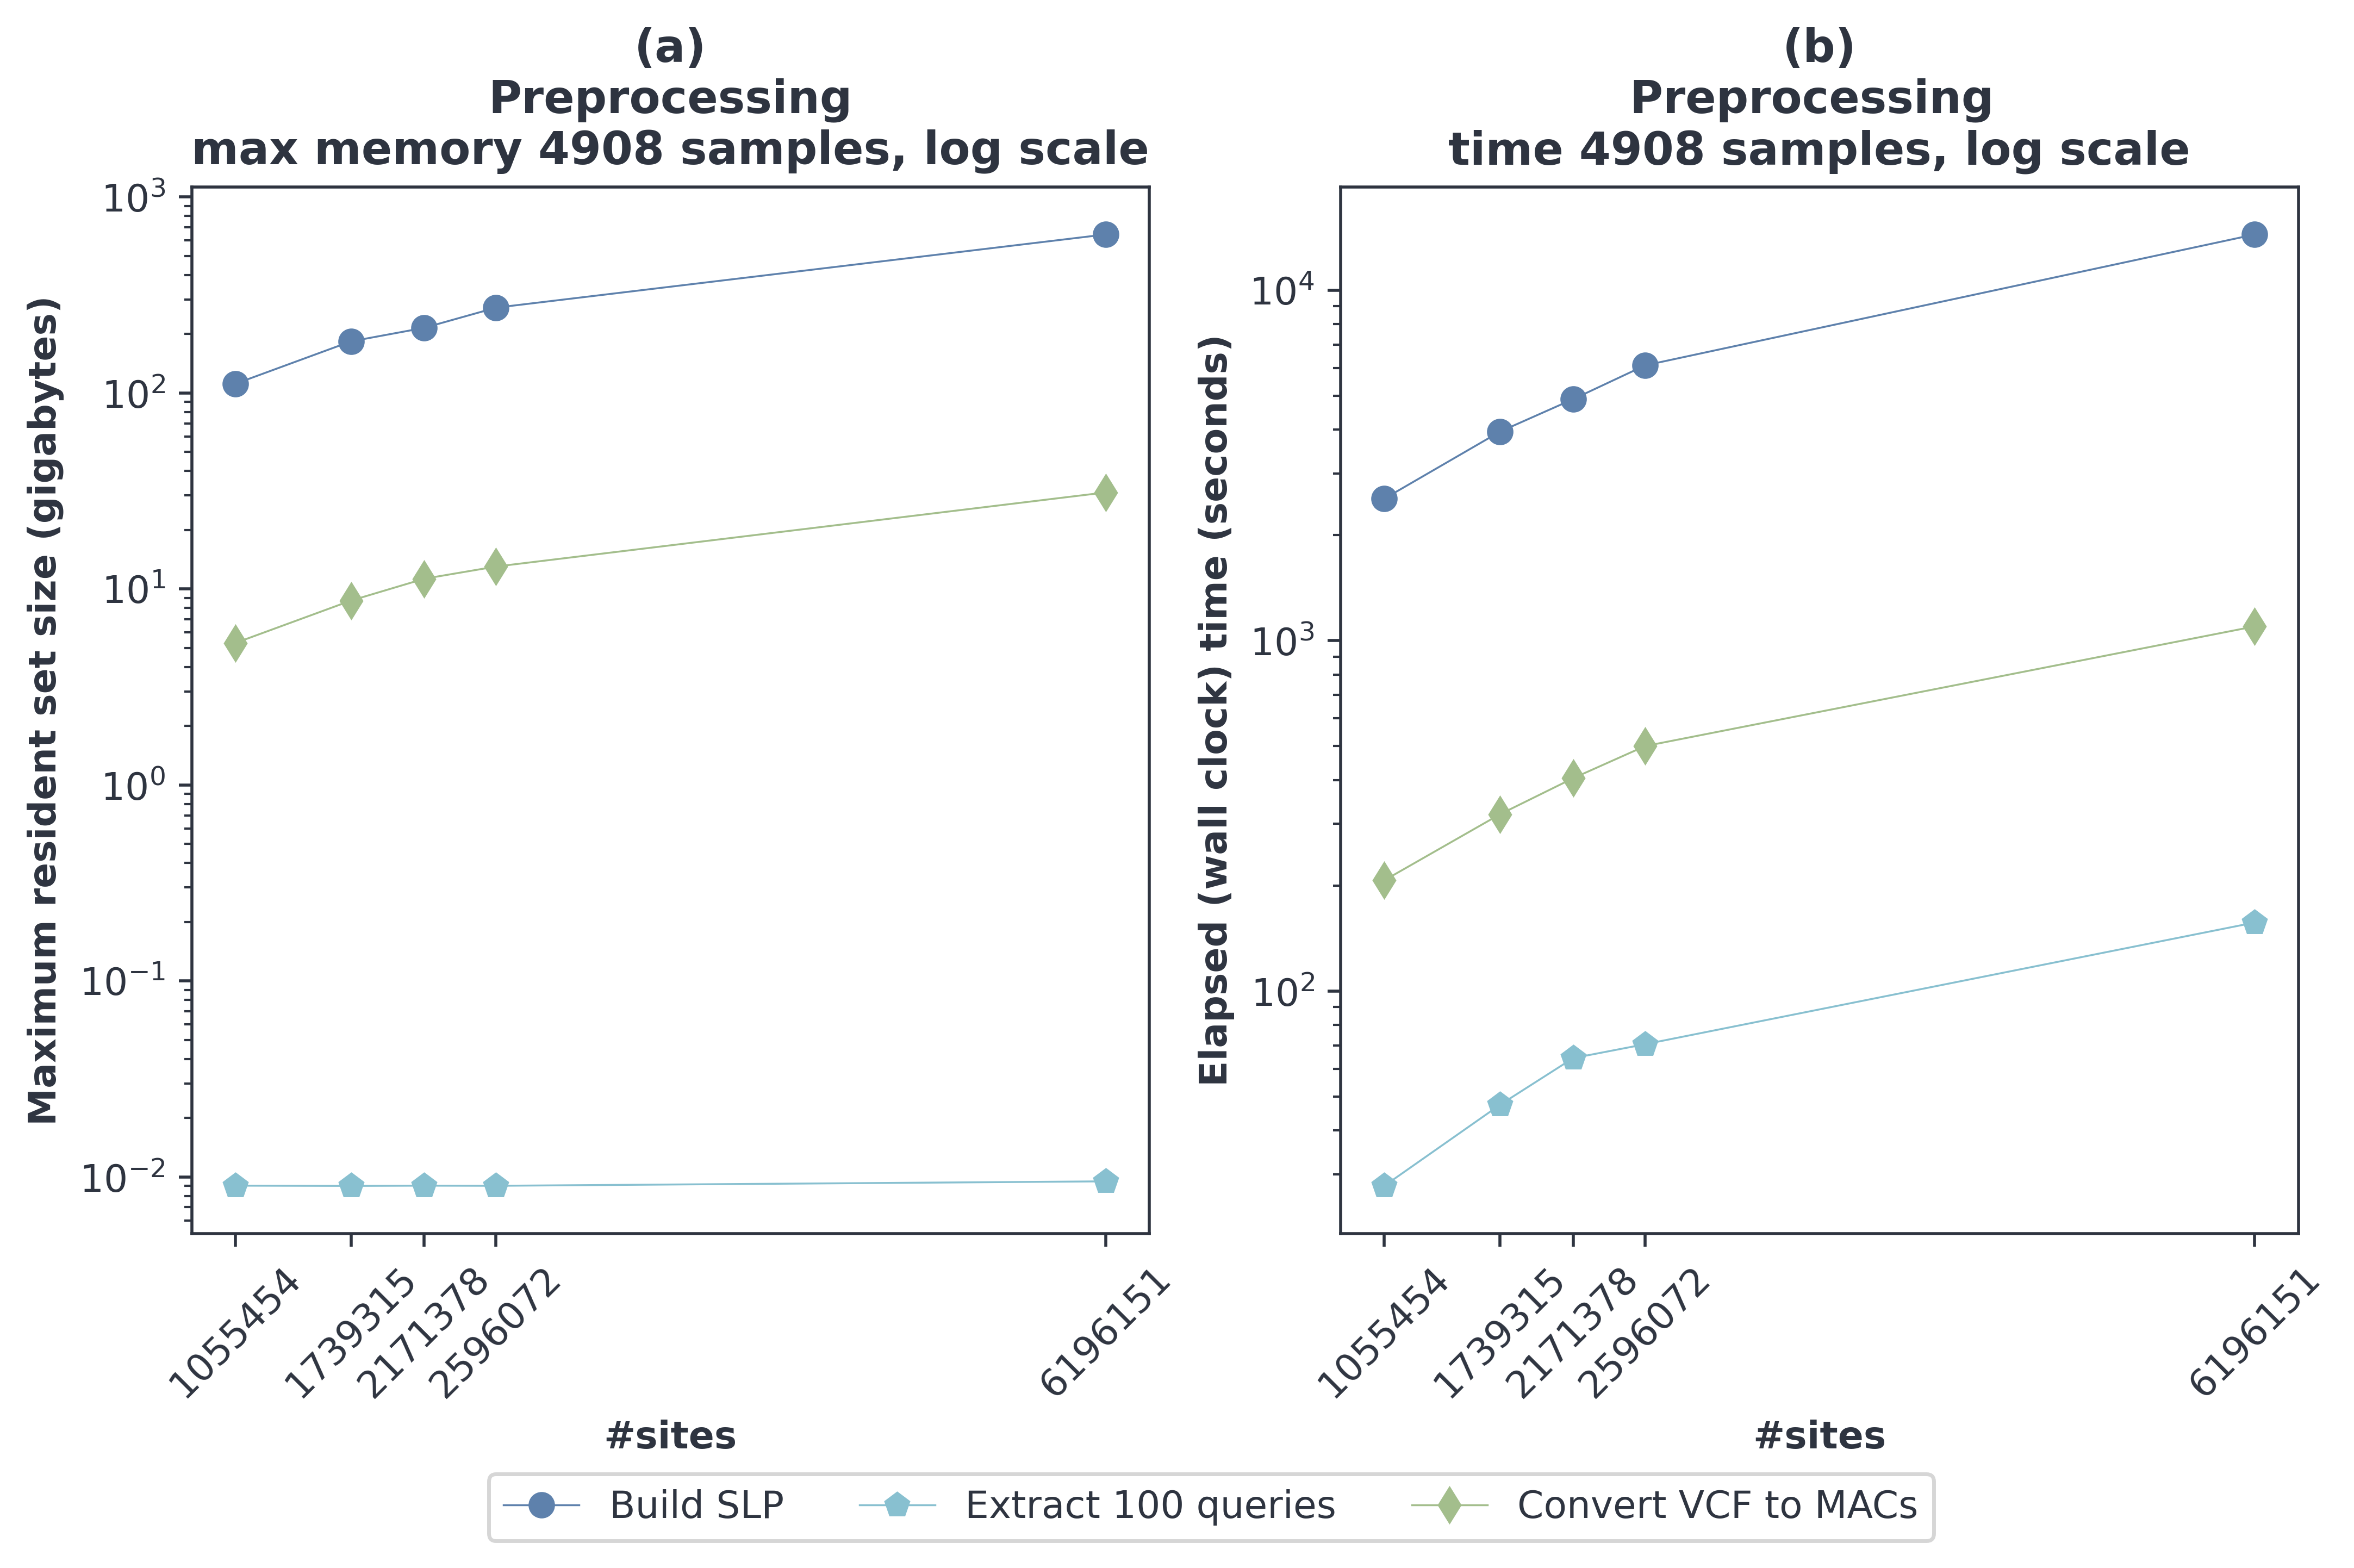
\includegraphics[width=\linewidth]{img/prep_mem_time.png}
  \caption{Picchi di memoria (a) e tempo richiesto (b) per le tre fasi di
    preprocessing dell'input per la \textit{RLPBWT}, in scala logaritmica.}
  \label{fig:prechr}
\end{figure}
\begin{table}
  \centering
  \small
  \caption{Risultati quantitivi dei picchi di memoria (gigabytes) relativi alle
    fasi di 
    preprocessing per l'input delle varianti della \textit{RLPBWT}}
  \label{tab:prepmem}
  \begin{tabular}{c||c|c|c}
    \textbf{Chr} & \textbf{Costruzione SLP} & \textbf{Conversione VCF a MACs}
    & \textbf{Estrazione query}\\
    \hline
    \hline
    chr22 & 111 & 5 & 0,0089  \\
    chr20 & 183 & 9 & 0,0090 \\
    chr18 & 215 & 11 & 0,0090 \\
    chr16 & 272 & 13 & 0,0090 \\
    chr1 & 644 & 31 & 0,0094 
  \end{tabular}
\end{table}
\begin{table}
  \centering
  \small
  \caption{Risultati quantitivi dei tempi (secondi) relativi alle fasi di
    preprocessing per l'input delle varianti della \textit{RLPBWT}}
  \label{tab:preptime}
  \begin{tabular}{c||c|c|c}
    \textbf{Chr} & \textbf{Costruzione SLP} & \textbf{Conversione VCF a MACs}
    & \textbf{Estrazione query}\\
    \hline
    \hline
    chr22 & 2542 & 207 & 28 \\
    chr20 & 3950 & 320 & 47 \\
    chr18 & 4890 & 405 & 64 \\
    chr16 & 6104 & 500 & 71 \\
    chr1 & 14430 & 1098 & 157
  \end{tabular}
\end{table}
In figura \ref{fig:slpmacschr} si può osservare il vantaggio in termini di
memoria che si ha con l'uso degli \textit{SLP}, confrontando il peso dei file
MACs con il peso delle grammatiche compresse. Si segnala, in ogni caso, che il
peso dei vari file MACs include anche i diversi header. In tabella
\ref{tab:slpmacs} si possono
confrontare quantitativamente tali risultati.
\begin{table}
  \centering
  \caption{Dimensioni, in gigabytes, degli \textit{SLP} e dei file \textit{MACs}
  per i vari pannelli del 1000 Genome Project.}
  \begin{tabular}{c||c|c|c}
    \textbf{Chr} & \textbf{SLP}
    & \textbf{MACs} & \textbf{\%}\\
    \hline
    \hline
    chr22 & 0,04 & 4,84 & 0,9\\
    chr20 & 0,06 & 7,98 & 0,76\\
    chr18 & 0,08 & 9,97 & 0,79\\
    chr16 & 0,1 & 11,91 & 0,81\\
    chr1 & 0,22 & 28,44 & 0,78\\
  \end{tabular}
  \label{tab:slpmacs}
\end{table}
È possibile, grazie a tali risultati, apprezzare la compressione di tali
grammatiche.  
Si noti che, essendo la capacità di compressione di un \textit{SLP}
direttamente correlata alle ripetizioni presenti nella stringa da comprimere, la
dimensione dell'\textit{SLP} non è perfettamente proporzionale al numero di siti
dei pannelli in analisi.
\begin{figure}
  \centering
  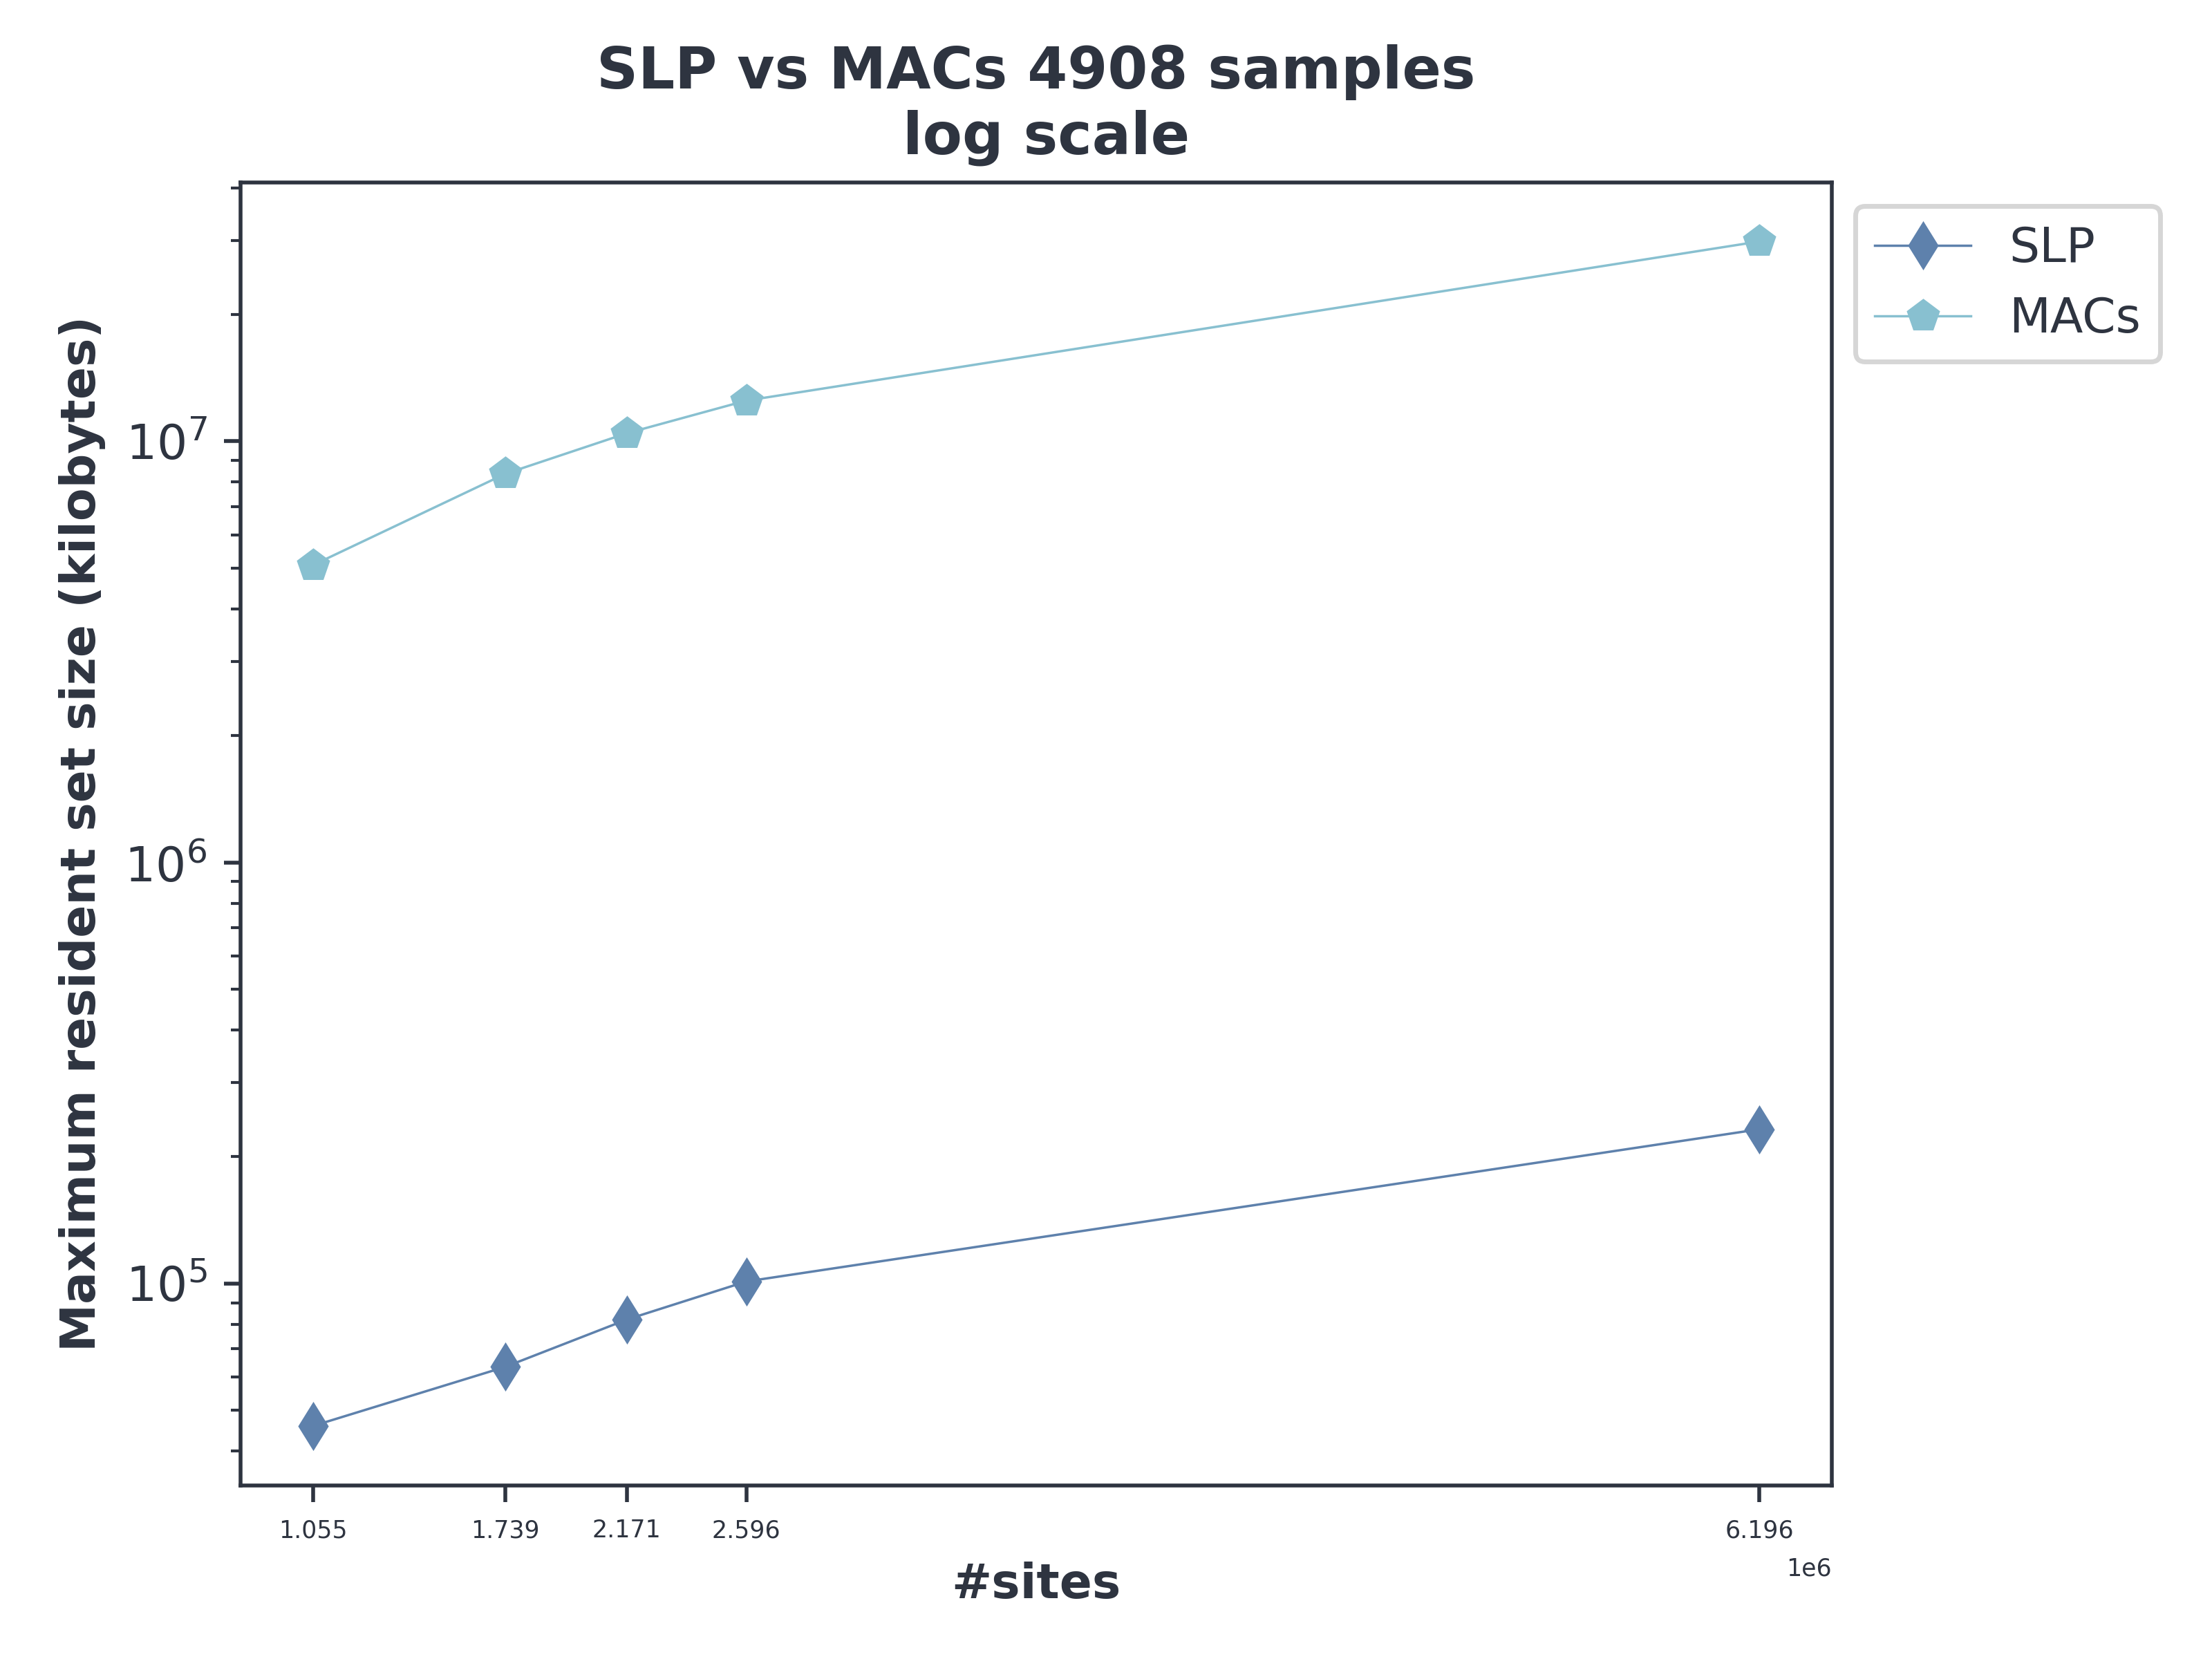
\includegraphics[width=0.7\linewidth]{img/slp_vs_macs_log.png}
  \caption{Confronto tra la memoria richiesta dai file MACs e dagli SLP per i
    pannelli del 1000 Genome Project, in scala
    logaritmica.} 
  \label{fig:slpmacschr}
\end{figure}
\paragraph{Costruzione della struttura.}
Passiamo ora ad analizzare tempi e picchi di memoria per la costruzione delle
strutture dati. Bisogna ricordare che:
\begin{itemize}
  \item nel caso della \textit{RLPBWT}, per ognuna delle strutture dati
  composte, questa fase prevede la costruzione e la 
  serializzazione dell'intera struttura dati
  \item nel caso della \textit{PBWT} questa fase crea unicamente un file
  compresso ad hoc, contenente le strutture base delle \textit{PBWT}. A partire
  da tale file, in fase di calcolo degli \textit{SMEM}, verranno calcolati anche
  tutti gli altri indici al calcolo degli stessi, a seconda dell'algoritmo usato
\end{itemize}
Fatte queste doverose premesse, passiamo ad analizzare i risultati.
In figura \ref{fig:maketimememchr} (a) vengono visualizzati i picchi di
memoria richiesti mentre in figura \ref{fig:maketimememchr} (b) i tempi di
calcolo delle strutture. Alla tabelle \ref{tab:makemem} e \ref{tab:maketime} si
riportano i risultati quantitativi in termini di gigabytes e secondi.\\ 
Come anticipato, l'implementazione della \textit{PBWT} non calcola e memorizza
tutti gli indici 
necessari al calcolo degli \textit{SMEM} in fase di costruzione, avendo quindi
una bassissima richiesta di memoria in questa fase. Discorso diverso si ha
parlando delle strutture dati per la \textit{RLPBWT}. Le strutture dati composte
\texttt{MAP-INT + LCP} e \texttt{MAP-BV + LCP}, dovendo 
memorizzare l'intero insieme degli \textit{array LCP}, hanno un elevato
consumo di memoria. Pur utilizzando degli \textit{int vector compressi}, in modo
analogo a quanto visto, ad esempio, per la componente \texttt{PERM}, si ha
necessità di salvare $NM$ valori interi, valori che, nel caso peggiore, sono
pari al numero di siti del pannello. Risulta ovvio notare come, in
termini di costruzione, siano le due strutture che non scalano sul numero di run
ad aver maggiori richieste di memoria. Proseguendo nell'analisi si ha che
l'utilizzo della componente 
\texttt{MAP-BV}, come atteso, richiede maggior memoria (approssimativamente tra
il 15\% e il 20\% in più) della componente
\texttt{MP-INT}. In merito invece ai tempi di costruzione delle due strutture si
segnala come i tempi di calcolo della componente \texttt{MAP-BV} siano superiori
rispetto a quelli della \texttt{MAP-INT} (anche in questo caso
approssimativamente tra il 15\% e il 20\% in più), dovendo, ad esempio, calcolare
anche le strutture per le funzioni \textit{rank/select} per i \textit{bitvector
  sparsi}. Nel caso della componente 
\texttt{MAP-INT}, invece, l'unica operazione aggiuntiva rispetto a quelle attese
per una classica popolazione di array di interi è la fase di compressione degli
stessi. Le analisi effettuate sulle componenti di \textit{mapping} sono da
ritenersi analoghe per le componenti dedicate alle \textit{threshold}, in
termini di uso di \textit{bitvector sparsi} e \textit{int vector
  compressi}. Tali considerazioni sono valide anche per le altre strutture
composte per la \textit{RLPBWT}. Infine, confrontando le strutture dati in grado
di computare l'array $MS$, si aggiungono le considerazioni sulle possibili
strutture per il \textit{random access} e, nel caso dell'\textit{SLP}, per l'uso
delle \textit{LCE query}. Si nota come l'uso della componente \texttt{RA-BV}
comporta, come atteso, una maggior richiesta di memoria, pur limitata dall'uso
dei \textit{bitvector}. Sempre in termini di tempi di esecuzione, si ha che la
componente \texttt{RA-BV} deve essere computata in fase di costruzione delle
strutture, comportando un aumento dei tempi di calcolo (meno del 5\% in
più). Confrontando i tempi di 
tutte le varianti si ha che tutti gli algoritmi di costruzione sono in tempo
proporzionale a $\mathcal{O}(NM)$ ma, come detto, le varianti della
\textit{RLPBWT} includono, in questa fase, anche il calcolo delle strutture
utili al calcolo degli SMEM. Si noti come, parlando di \textit{RLPBWT}, la
struttura composta \texttt{MAP-INT + LCE + PERM + PHI} risulti essere la meno
costosa in termini di memoria, usando la struttura di mapping tramite
\textit{int vector compressi} e l'\textit{SLP} (per le \textit{LCE
  query}). Anche in termini di tempo, per i discorsi fatti sui tempi di calcolo
delle singole componenti, risulta essere la soluzione più vantaggiosa.\\
In generale, si può 
concludere che questa frase conferma quanto discusso nel capitolo
\ref{metchap}.\\ 
\begin{figure}
  \centering
  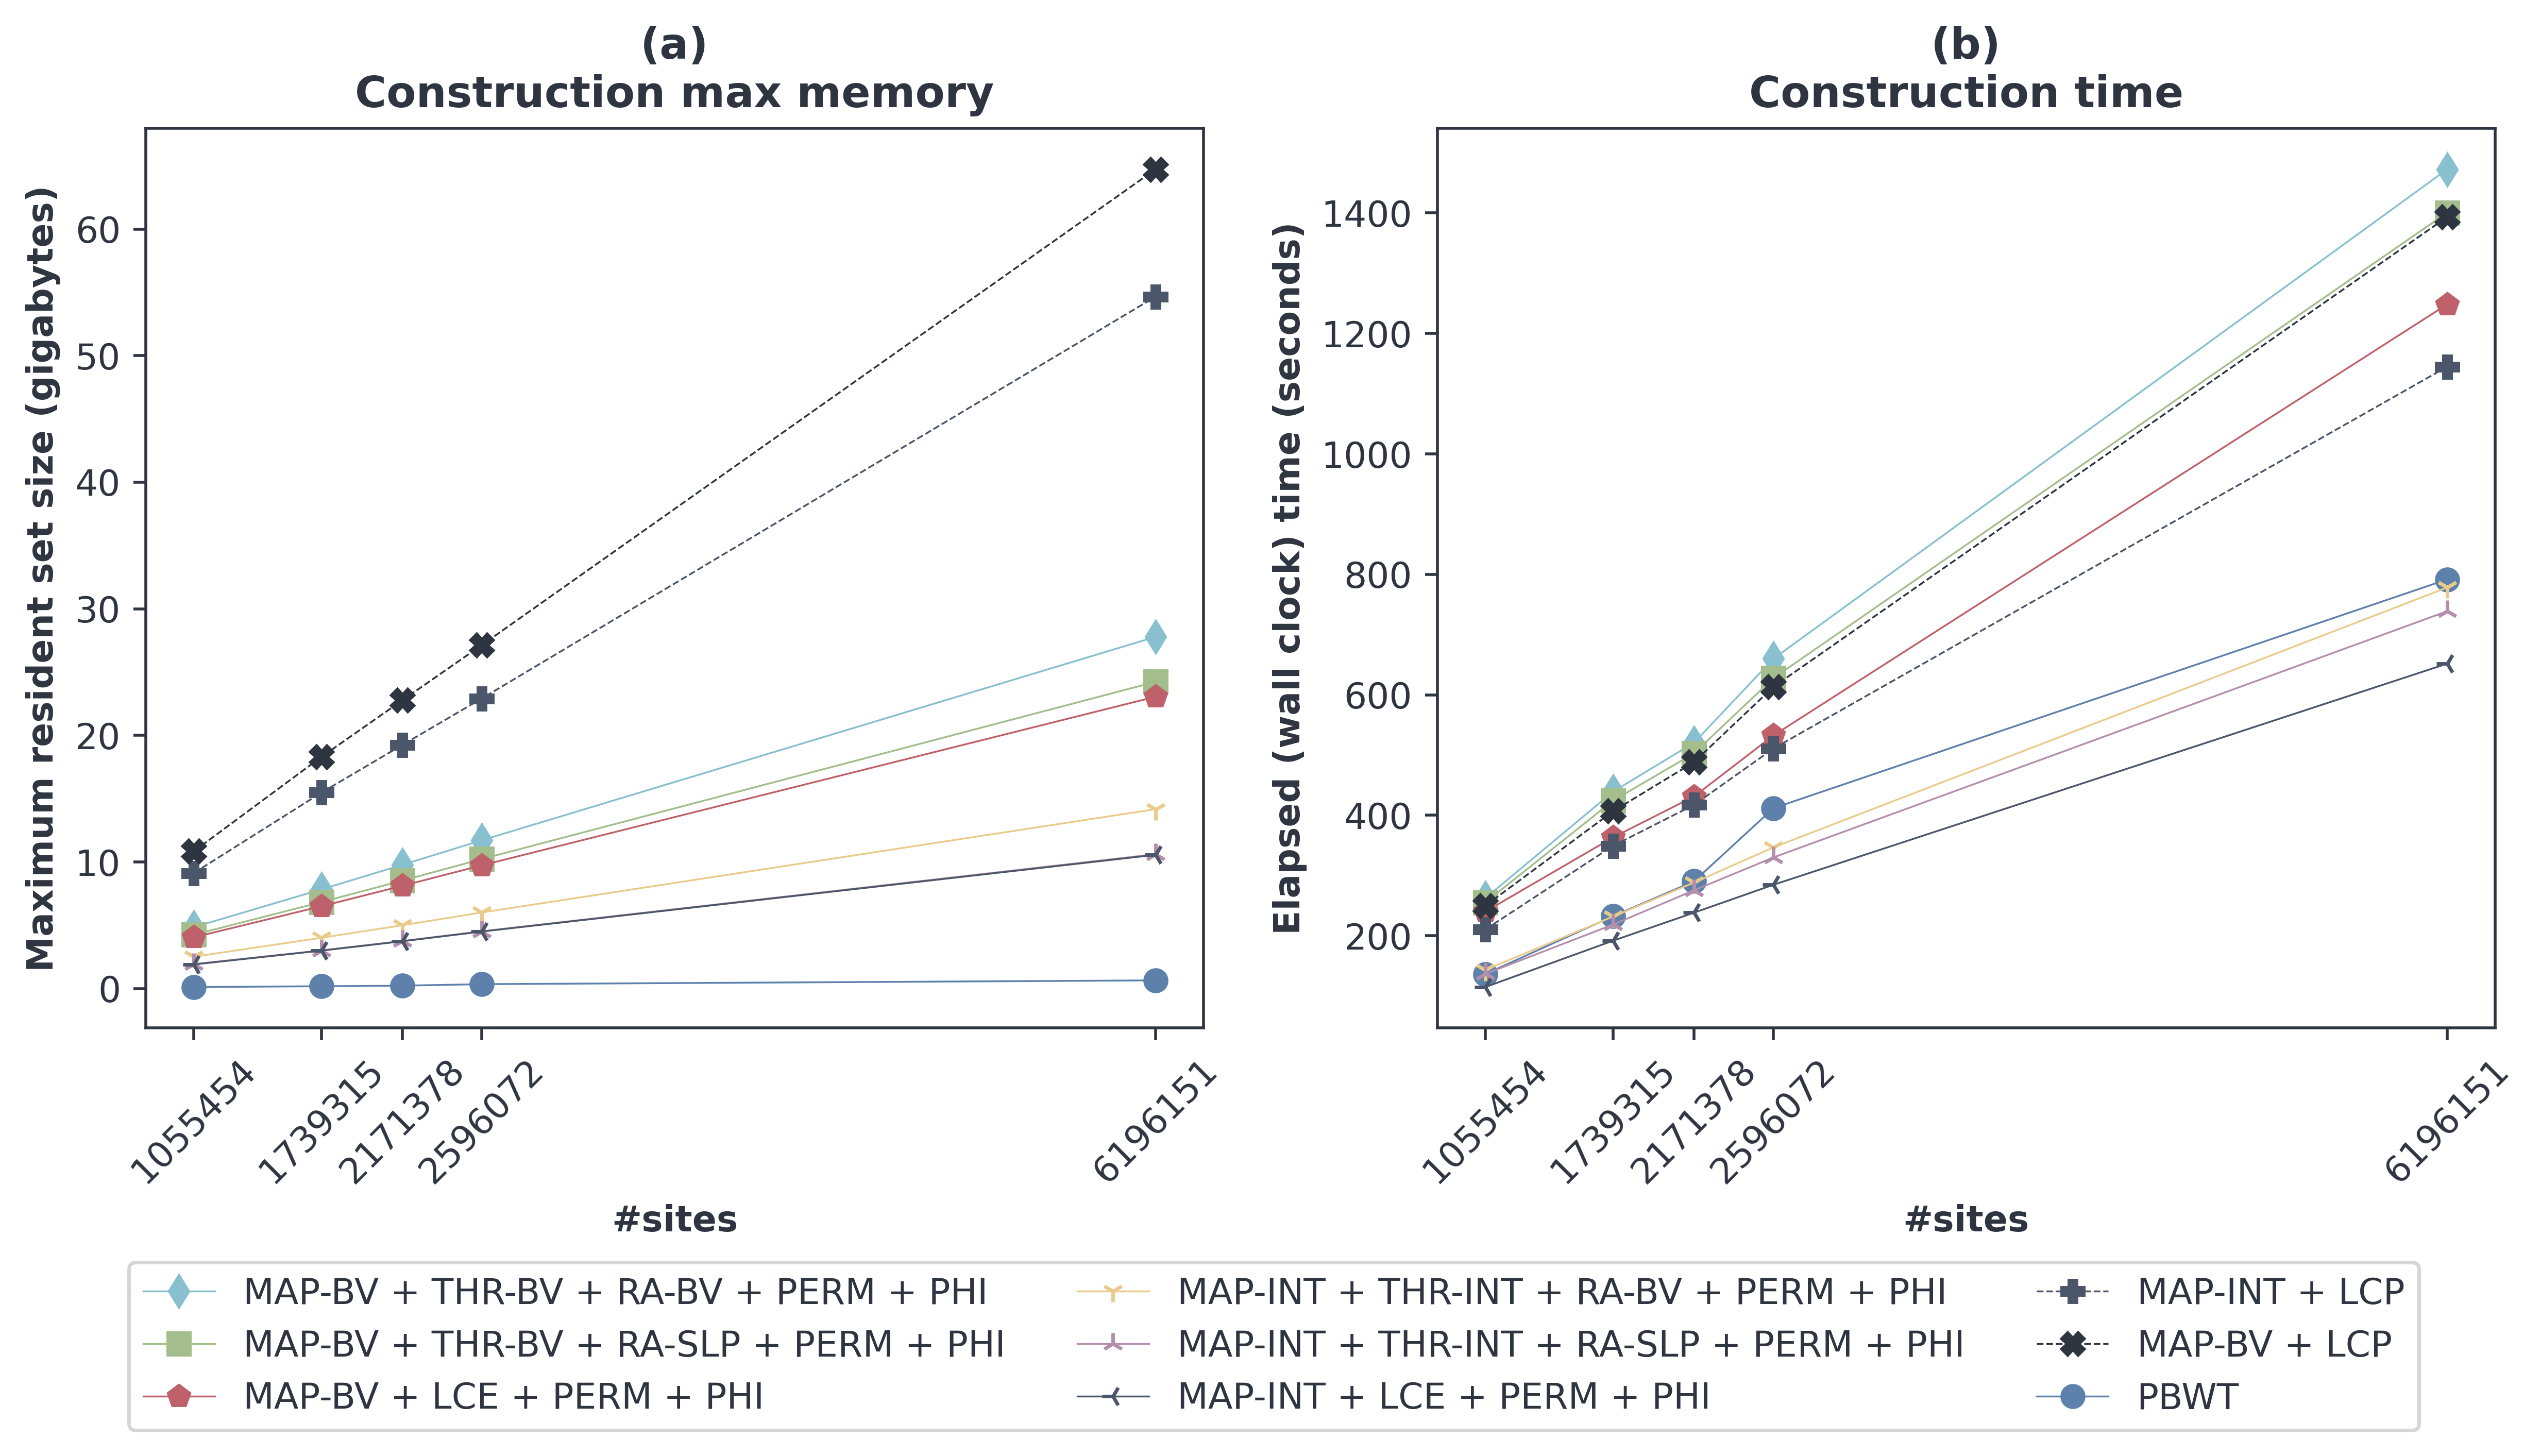
\includegraphics[width=\linewidth]{img/make_time_mem_paper.png}
  \caption{Picchi di memoria (a) e tempi di calcolo (b) per la
    costruzione delle varianti della RLPWBT e per 
    la PBWT.}
  \label{fig:maketimememchr}
\end{figure}
\begin{table}
  \centering
  \caption{Risultati quantitativi dei picchi di memoria (gigabytes) di
    costruzione delle 
    strutture dati.} 
  \label{tab:makemem}
  \footnotesize
  \subcaption*{\footnotesize{Tabella A: risultati relativi alla \textit{PBWT} e
      alle varianti 
    basate su \texttt{LCP} per la \textit{RLPBWT}.}} 
  \begin{tabular}{c||c|c|c} 
    \textbf{Chr}
    & \textbf{PBWT}
    & \textbf{\texttt{MAP-INT \newline+ LCP}}
    & \textbf{\texttt{MAP-BV \newline+ LCP}}\\
    \hline
    \hline
    chr22 & 0.1 & 9 & 11  \\
    chr20 & 0.2 & 15 & 18 \\
    chr18 & 0.2 & 19 & 23 \\
    chr16 & 0.3 & 23 & 27 \\
    chr1 & 0.6 & 55 & 65  \\
  \end{tabular}
  \vspace{+3mm}
  \subcaption*{\footnotesize{Tabella B: risultati relativi alle varianti basate
      su 
      \textit{matching statistics} e \textit{bitvector sparsi} per la
      \textit{RLPBWT}.}}
  \vspace{+1mm}
  \begin{tabular}{c||c|c|c} 
    \textbf{Chr}
    & \textbf{\texttt{MAP/THR-BV + RA-BV $\cdots$}}
    & \textbf{\texttt{MAP/THR-BV + RA-SLP$\cdots$}}
    & \textbf{\texttt{MAP-BV + LCE $\cdots$}}\\
    \hline
    \hline
    chr22 & 5 & 4 & 4 \\
    chr20 & 8 & 7 & 7 \\
    chr18 & 10 & 9 & 8  \\
    chr16 & 12 & 10 & 10 \\
    chr1 & 28 & 24 & 23 \\
  \end{tabular}
  \vspace{+3mm}
  \subcaption*{\footnotesize{Tabella C: risultati relativi alle varianti basate
      su 
    \textit{matching statistics} e \textit{int vector compressi} per la
    \textit{RLPBWT}.}}
  \vspace{+1mm}
  \begin{tabular}{c||c|c|c} 
    \textbf{Chr}
    & \textbf{\texttt{MAP/THR-INT + RA-BV $\cdots$}}
    & \textbf{\texttt{MAP/THR-INT + RA-SLP $\cdots$}}
    & \textbf{\texttt{MAP-INT + LCE $\cdots$}}\\
    \hline
    \hline
    chr22 & 3 & 2 & 2 \\
    chr20 & 4 & 3 & 3 \\
    chr18 & 5 & 4 & 4 \\
    chr16 & 6 & 5 & 5 \\
    chr1 & 14 & 12 & 11 
  \end{tabular}
\end{table}
\begin{table}
  \centering
  \caption{Risultati quantitativi dei tempi (secondi) di costruzione delle
    strutture dati.} 
  \label{tab:maketime}
  \footnotesize
  \subcaption*{\footnotesize{Tabella A: risultati relativi alla \textit{PBWT} e
      alle varianti 
    basate su \texttt{LCP} per la \textit{RLPBWT}.}} 
  \begin{tabular}{c||c|c|c} 
    \textbf{Chr}
    & \textbf{PBWT}
    & \textbf{\texttt{MAP-INT \newline+ LCP}}
    & \textbf{\texttt{MAP-BV \newline+ LCP}}\\
    \hline
    \hline
    chr22 & 136 & 210 & 250 \\
    chr20 & 233 & 349 & 407 \\
    chr18 & 290 & 417 & 488 \\
    chr16 & 412 & 511 & 613 \\
    chr1 & 792 & 1145 & 1393
  \end{tabular}
  \vspace{+3mm}
  \subcaption*{\footnotesize{Tabella B: risultati relativi alle varianti basate
      su 
      \textit{matching statistics} e \textit{bitvector sparsi} per la
      \textit{RLPBWT}.}}
  \vspace{+1mm}
  \begin{tabular}{c||c|c|c} 
    \textbf{Chr}
    & \textbf{\texttt{MAP/THR-BV + RA-BV $\cdots$}}
    & \textbf{\texttt{MAP/THR-BV + RA-SLP $\cdots$}}
    & \textbf{\texttt{MAP-BV + LCE $\cdots$}}\\
    \hline
    \hline
    chr22 & 262 & 255 & 240 \\
    chr20 & 439 & 424 & 363 \\
    chr18 & 521 & 503 & 431 \\
    chr16 & 660 & 628 & 533 \\
    chr1 & 1472 & 1400 & 1248 
  \end{tabular}
  \vspace{+3mm}
  \subcaption*{\footnotesize{Tabella C: risultati relativi alle varianti basate
      su 
    \textit{matching statistics} e \textit{int vector compressi} per la
    \textit{RLPBWT}.}}
  \vspace{+1mm}
  \begin{tabular}{c||c|c|c} 
    \textbf{Chr}
    & \textbf{\texttt{MAP/THR-INT + RA-BV $\cdots$}}
    & \textbf{\texttt{MAP/THR-INT + RA-SLP $\cdots$}}
    & \textbf{\texttt{MAP-INT + LCE $\cdots$}}\\
    \hline
    \hline
    chr22 & 143 & 137 & 115 \\
    chr20 & 232 & 219 & 192 \\
    chr18 & 288 & 275 & 238 \\
    chr16 & 347 & 330 & 285 \\
    chr1 & 778 & 739 & 652

  \end{tabular}
\end{table}
\dc{Controllare tutti questi dati}
Sfruttando i metodi offerti da \textit{SDSL-LITE}, è possibile studiare
l'occupazione di memoria delle singole componenti trattate nel capitolo
\ref{metchap}. 
In tabella \ref{tab:comp} e in figura \ref{fig:comp}
si riportano, in megabytes, 
le dimensioni di tali componenti. Si può,
innanzitutto, apprezzare il vantaggio dell'uso della componente
\texttt{RA-SLP/LCE} rispetto alla 
componente \texttt{RA-BV}, avendo che si ha un risparmio di memoria superiore al
90\%. Numericamente tale vantaggio è riportato in tabella
\ref{tab:slppanel}.
\begin{table}
  \centering
  \caption{Vantaggio percentuale dell'uso delle componenti \texttt{RA-SLP/LCE}
    rispetto alla componente \texttt{RA-BV}.}
  \begin{tabular}{c||c|c|c}
    \textbf{Chr} & \textbf{\texttt{RA-SLP/LCE}
                                          (\textit{MB})}
    & \textbf{\texttt{RA-BV} (\textit{MB})} & \textbf{\%}\\
    \hline
    \hline
    chr22 & 44 & 628 & 7\\
    chr20 & 61 & 1.035 & 6\\
    chr18 & 80 & 1.292 & 6\\
    chr16 & 98 & 1.544 & 6\\
    chr1 & 226 & 3.687 & 6\\
  \end{tabular}
  \label{tab:slppanel}
\end{table}
Confermando nuovamente quando detto diverse volte nella tesi, si segnala il
forte vantaggio in memoria nell'utilizzo delle componenti basate su \textit{int
  vector compressi}, rispetto che a quelle basate su \textit{sparse
  bitvector}.\\
Si nota, infine, come le componenti \texttt{PERM} e \texttt{PHI}, non
presentino particolari criticità dal punto di vista della memoria
richiesta. Infine, terminando l'analisi di tali risultati, senza trattare
nuovamente le componenti per il \textit{random access}, si ha conferma della
richiesta eccessiva in memoria della componente \texttt{LCP}.
\dc{Serve altro?}
\begin{figure}
  \centering
    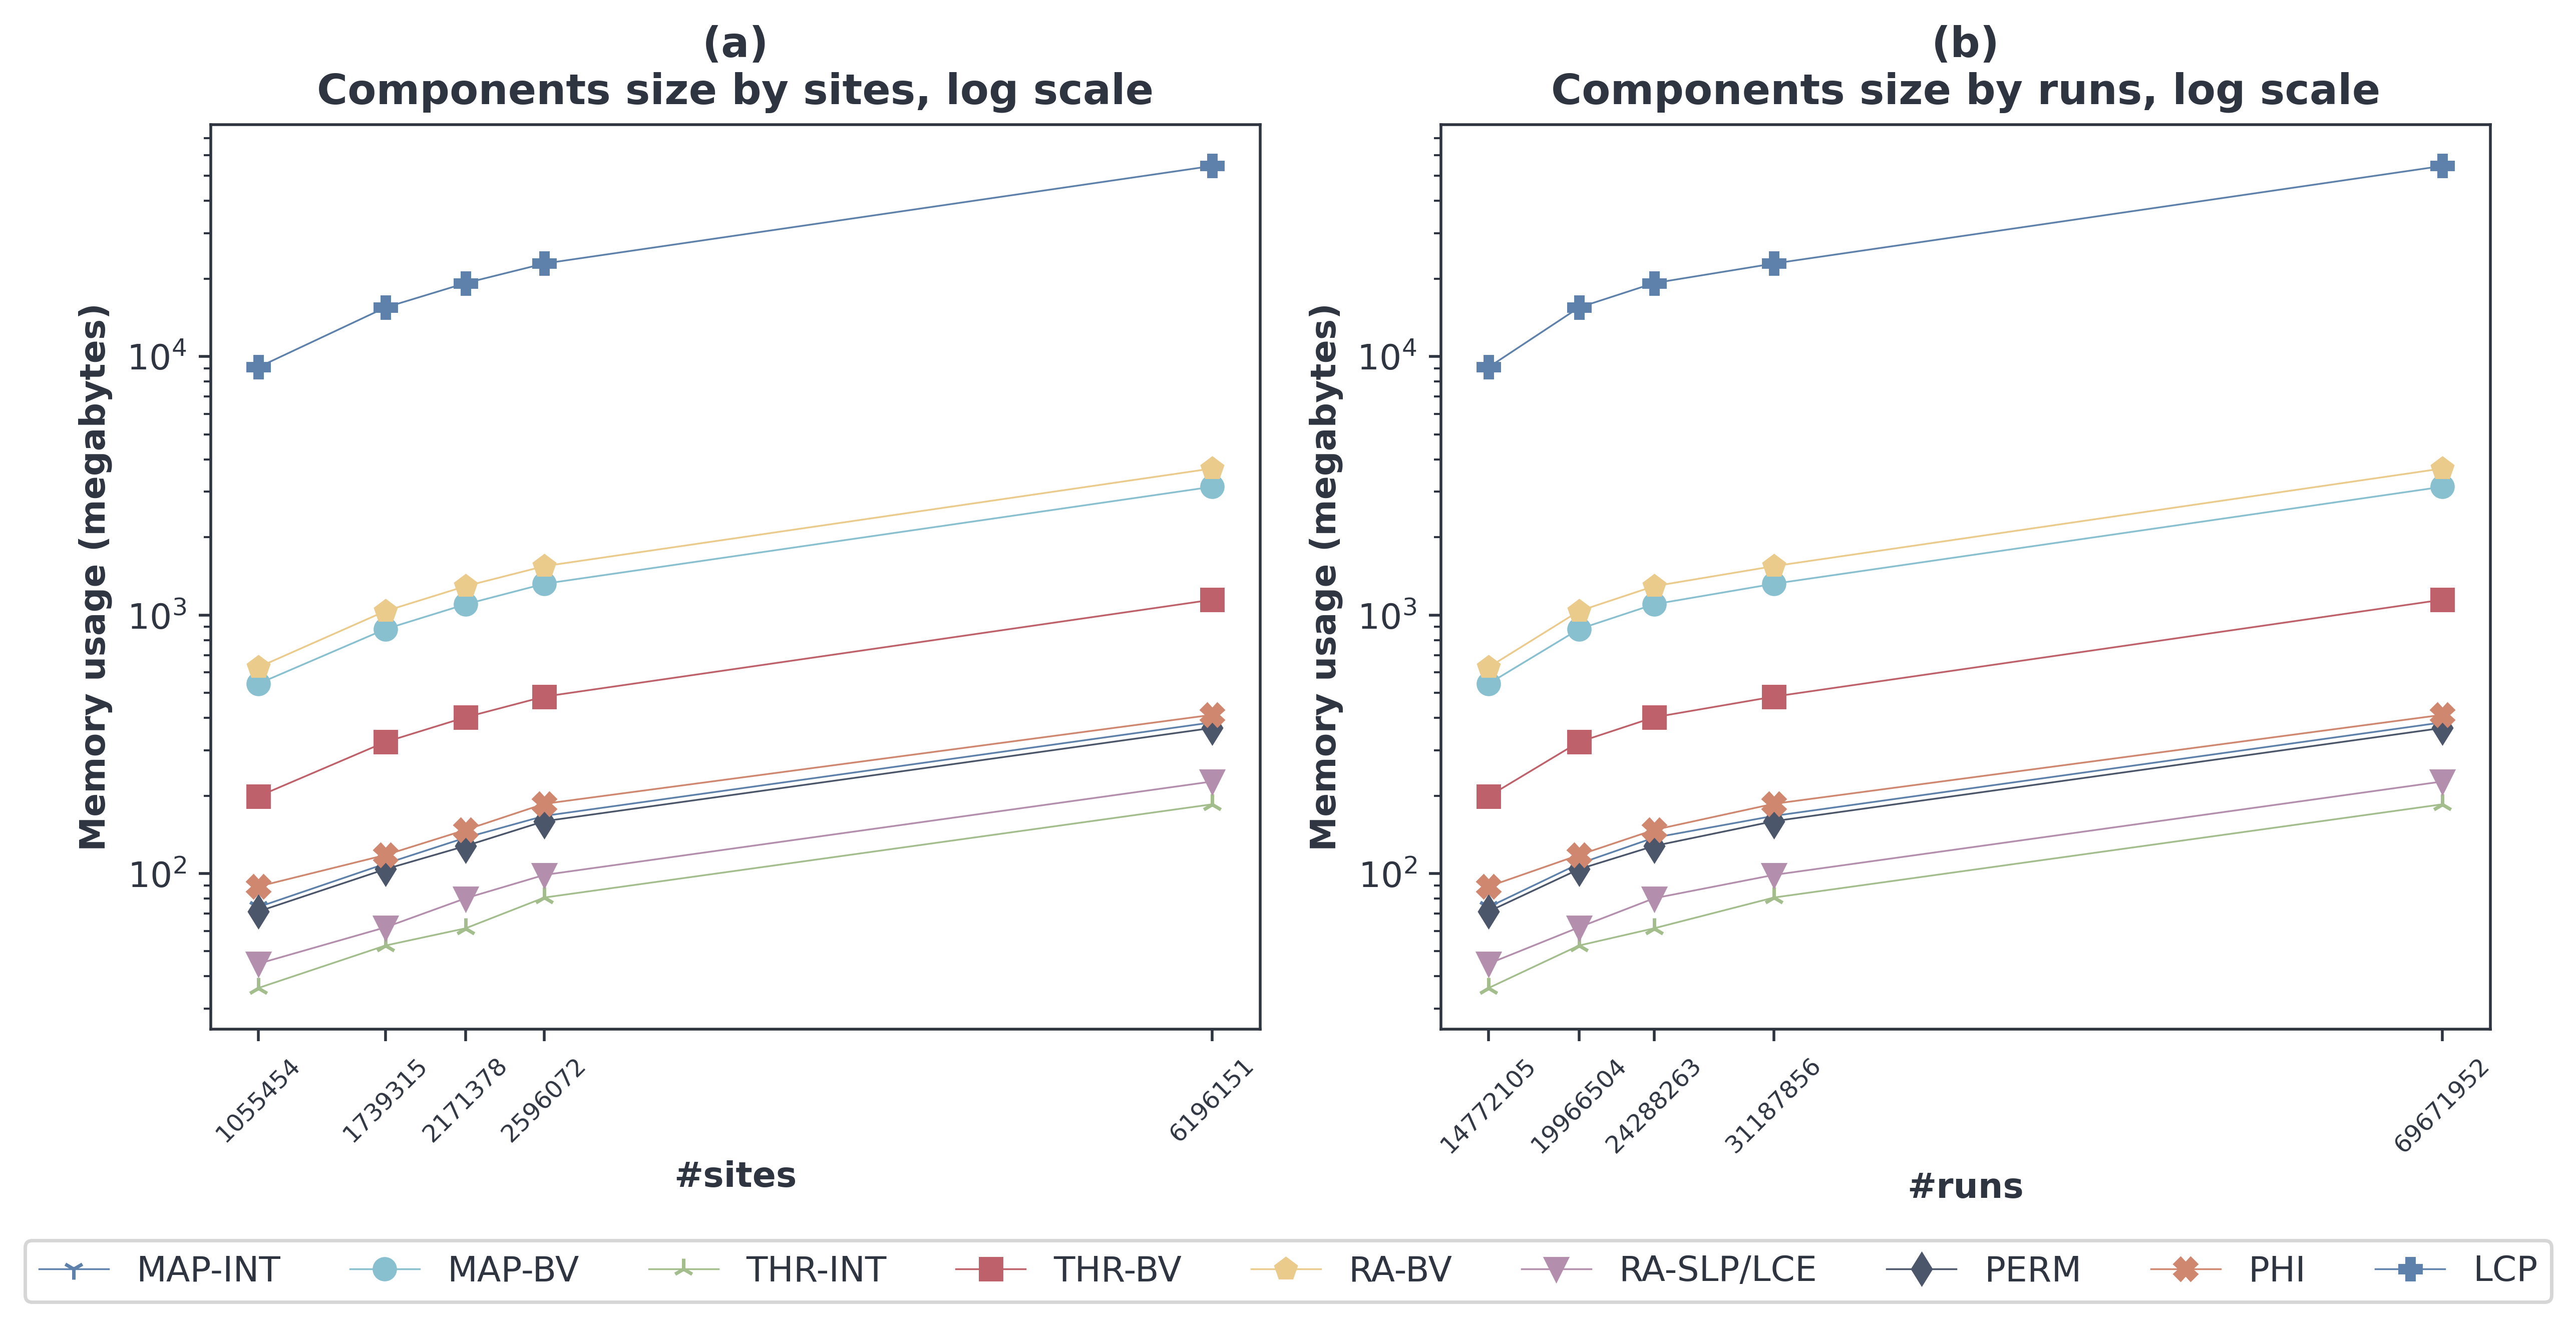
\includegraphics[width=\linewidth]{img/comp_mem.png}
  \caption{Memoria occupata dalle singole componenti, avendo sulle ascisse in
    (a) il numero di siti e in (b) il numero di run. }
  \label{fig:comp}
\end{figure}
\begin{table}
  \centering
  \caption{Dimensioni, in megabytes, delle singole componenti per la
    \textit{RLPBWT}.} 
  \label{tab:comp}
  \subcaption*{\footnotesize{Tabella A: dimensioni delle componenti di
    \textit{mapping} e \textit{threshold} usate nelle
    strutture dati per la \textit{RLPBWT}.}}   
  \begin{tabular}{c||c|c|c|c}
    \textbf{Chr} & \textbf{\texttt{MAP-INT}} & \textbf{\texttt{MAP-BV}}
    & \textbf{\texttt{THR-INT}} & \textbf{\texttt{THR-BV}} \\
    \hline
    \hline
    22 & 74 & 543 & 36 & 199\\ \hline
    20 & 109 & 882 & 53 & 322\\ \hline
    18 & 137 & 1.100 & 61 & 402\\ \hline
    16 & 167 & 1.320 & 81 & 483\\ \hline
    1 & 384 & 3.133 & 185 & 1.146
  \end{tabular}
  \vspace{+3mm}
  \subcaption*{\footnotesize{Tabella B: dimensioni delle componenti di
      \textit{random access}, \textit{prefix array samples} e \textit{struttura
      $\phi$}.} }
 \vspace{+1mm}
  \begin{tabular}{c||c|c|c|c|c}
    \textbf{Chr} & \textbf{\texttt{RA-BV}} & \textbf{\texttt{RA-SLP/LCE}}
    & \textbf{\texttt{PERM}} & \textbf{\texttt{PHI}} & \textbf{\texttt{LCP}}\\
    \hline
    \hline
    22 & 628 & 44 & 71 & 89 & 9.095\\ \hline
    20 & 1.035 & 62 & 104 & 118 & 15.468 \\ \hline
    18 & 1.292 & 80 & 128 & 147 & 19.223 \\ \hline
    16 & 1.545 & 99 & 159 & 186 & 22.888\\ \hline
    1 & 3.687 & 227 & 366 & 411 & 54.588
  \end{tabular}
\end{table}
\paragraph{Calcolo degli SMEM.}
In seguito si ha la discussione dei risultati ottenuti per il calcolo degli
\textit{SMEM}.\\ 
In figura \ref{fig:smemtimememchr} (a) si riportano i risultati i termini di
picchi di 
memoria durante la computazione degli \textit{SMEM}. Tali risultati sono
consultabili numericamente in tabella \ref{tab:exemem}. Come previsto,
l'algoritmo 
\texttt{matchDynamic} della \textit{PBWT} ha le migliori prestazioni
in spazio, calcolando dinamicamente i vari indici necessari al calcolo degli
\textit{SMEM ``interni''}. D'altro canto per quanto riguarda l'\textit{algoritmo
  5} di Durbin, ovvero l'algoritmo \texttt{matchIndexed}, si confermano le
previsioni 
fatte dall'autore stesso, avendo che la memoria utilizzata è circa $13NM$
bytes. Escludendo le strutture \texttt{MAP-INT + LCP} e \texttt{MAP-BV + LCP},
si parla di circa un'intero ordine di grandezza in più di memoria rispetto alle
strutture dati composte per la \textit{RLPBWT}. Parlando di queste ultime, la
differenza tra le varie strutture dati che supportano il calcolo 
dell'array $MS$ è dovuta, a parità di componente per il mapping (e
conseguentemente della componente per le threshold), dall'uso della componente
\texttt{RA-BV} o della componente \texttt{RA-SLP} (o della componente
\texttt{LCE}), in modo analogo a quanto visto discutendo il peso in memoria
delle singole componenti.\\
% Interessante è notare il rapporto tra la memoria richiesta dalla \textit{RLPBWT}
% con \textit{SLP} e \textit{LCE} e la \textit{PBWT Indexed}:
% \begin{table}[H]
%   \centering
%   \footnotesize
%   \begin{tabular}{c|c|c|c|c}
%     \textbf{\#Samples} & \textbf{\#Siti}
%     & \textbf{RLPBWT SLP-LCE (\textit{kb})}
%     & \textbf{PBWT Indexed (\textit{kb})} & \textbf{\%}\\
%     \hline
%     4908 & 1055454 & 3058088 & 65975520 & 4.64\\
%     4908 & 1739315 & 4961664 & 108713424 & 4.56\\
%     4908 & 2171378 & 6190684 & 135726084 & 4.56\\
%     4908 & 2596072 & 7430300 & 162257008 & 4.58\\
%     4908 & 6196151 & 17635700 & 387252160 & 4.55
%   \end{tabular}
% \end{table}
% Anche in questo caso le percentuali risultano leggermente peggiori rispetto ai
% pannelli simulati, pur restando risultati molto interessanti.
In figura \ref{fig:smemtimememchr} (b) si riportano, invece, i risultati i
termini di tempo di calcolo. Tali risultati sono
consultabili numericamente in tabella \ref{tab:exetime}. Anche in questo caso
l'algoritmo 
\texttt{matchDynamic} risulta essere il più performante, in quanto studia
contemporaneamente l'intero pannello di query. Parlando di \textit{RLPBWT},  la
struttura \texttt{MAP-INT + THR-INT + RA-SLP + PERM + PHI} e la 
struttura 
\texttt{MAP-BV + THR-BV + RA-SLP + PERM + PHI}, a causa delle
frequenti operazioni di \textit{random access} con la componente
\texttt{RA-SLP}, sia per il calcolo delle lunghezze delle 
matching statistics che per la fase di ``disambiguazione'', richiede più tempo
di tutte le altre varianti, soprattutto se si pensa alla corrispondente
variante con componente \texttt{RA-BV}. L'uso della componente \texttt{RA-SLP}
comporta, infatti, circa venti volte i tempi di calcolo usando i
\textit{bitvector sparsi} e addirittura di circa 45 volte usando gli
\textit{int vector compressi}. La struttura \texttt{MAP-INT + LCE +
  PERM + PHI} e la struttura 
\texttt{MAP-BV + LCE + PERM + PHI} risultano essere, al massimo,
il doppio più lenta rispetto all'algoritmo \texttt{matchIndexed}, con una
differenze che diventa quasi trascurabile all'aumentare delle dimensioni del
pannello. Questo è un 
risultato molto interessante se si tiene in considerazione la memoria necessaria
per il calcolo degli \textit{SMEM}.\\
Confrontando l'uso delle \textit{LCE query} con l'uso della componente
\texttt{RA-BV} si hanno, invece, tempi triplicati nel caso di \textit{mapping} e
\textit{threshold} con \textit{bitvector sparsi}. Nel caso degli \textit{int
  vector compressi} si hanno, d'altro canto, circa sette volte i tempi di
computazione. A priori delle componenti per \textit{mapping} e
\textit{threshold}, l'uso della componente \texttt{RA-SLP} comporta circa sei
volte il tempo d'uso delle \textit{LCE query}. Queste ultime analisi comportano
che l'uso del \textit{random access} su \textit{SLP} è la peggior soluzione in
ottica calcolo delle \textit{matching statistics}.\\
Concludendo, si può notare come la struttura composta
\texttt{MAP-INT + THR-INT + RA-BV + PERM + PHI}, tra quelle per la
\textit{RLPBWT}, risulti essere la migliore in termini di tempi di calcolo
mentre la struttura composta \texttt{MAP-INT + LCE + PERM + PHI} sia la
migliore in termini di memoria richiesta. Notando come quest'ultima sia circa 10
volte più lenta si può inferire come la scelta della miglior soluzione per la
\textit{RLPBWT} debba ricadere sulla \texttt{MAP-INT + THR-INT + RA-BV + PERM +
  PHI}, salvo situazioni in il risparmio di memoria sia un limite fondamentale
in fase di analisi dati. 
\begin{figure}
  \centering
  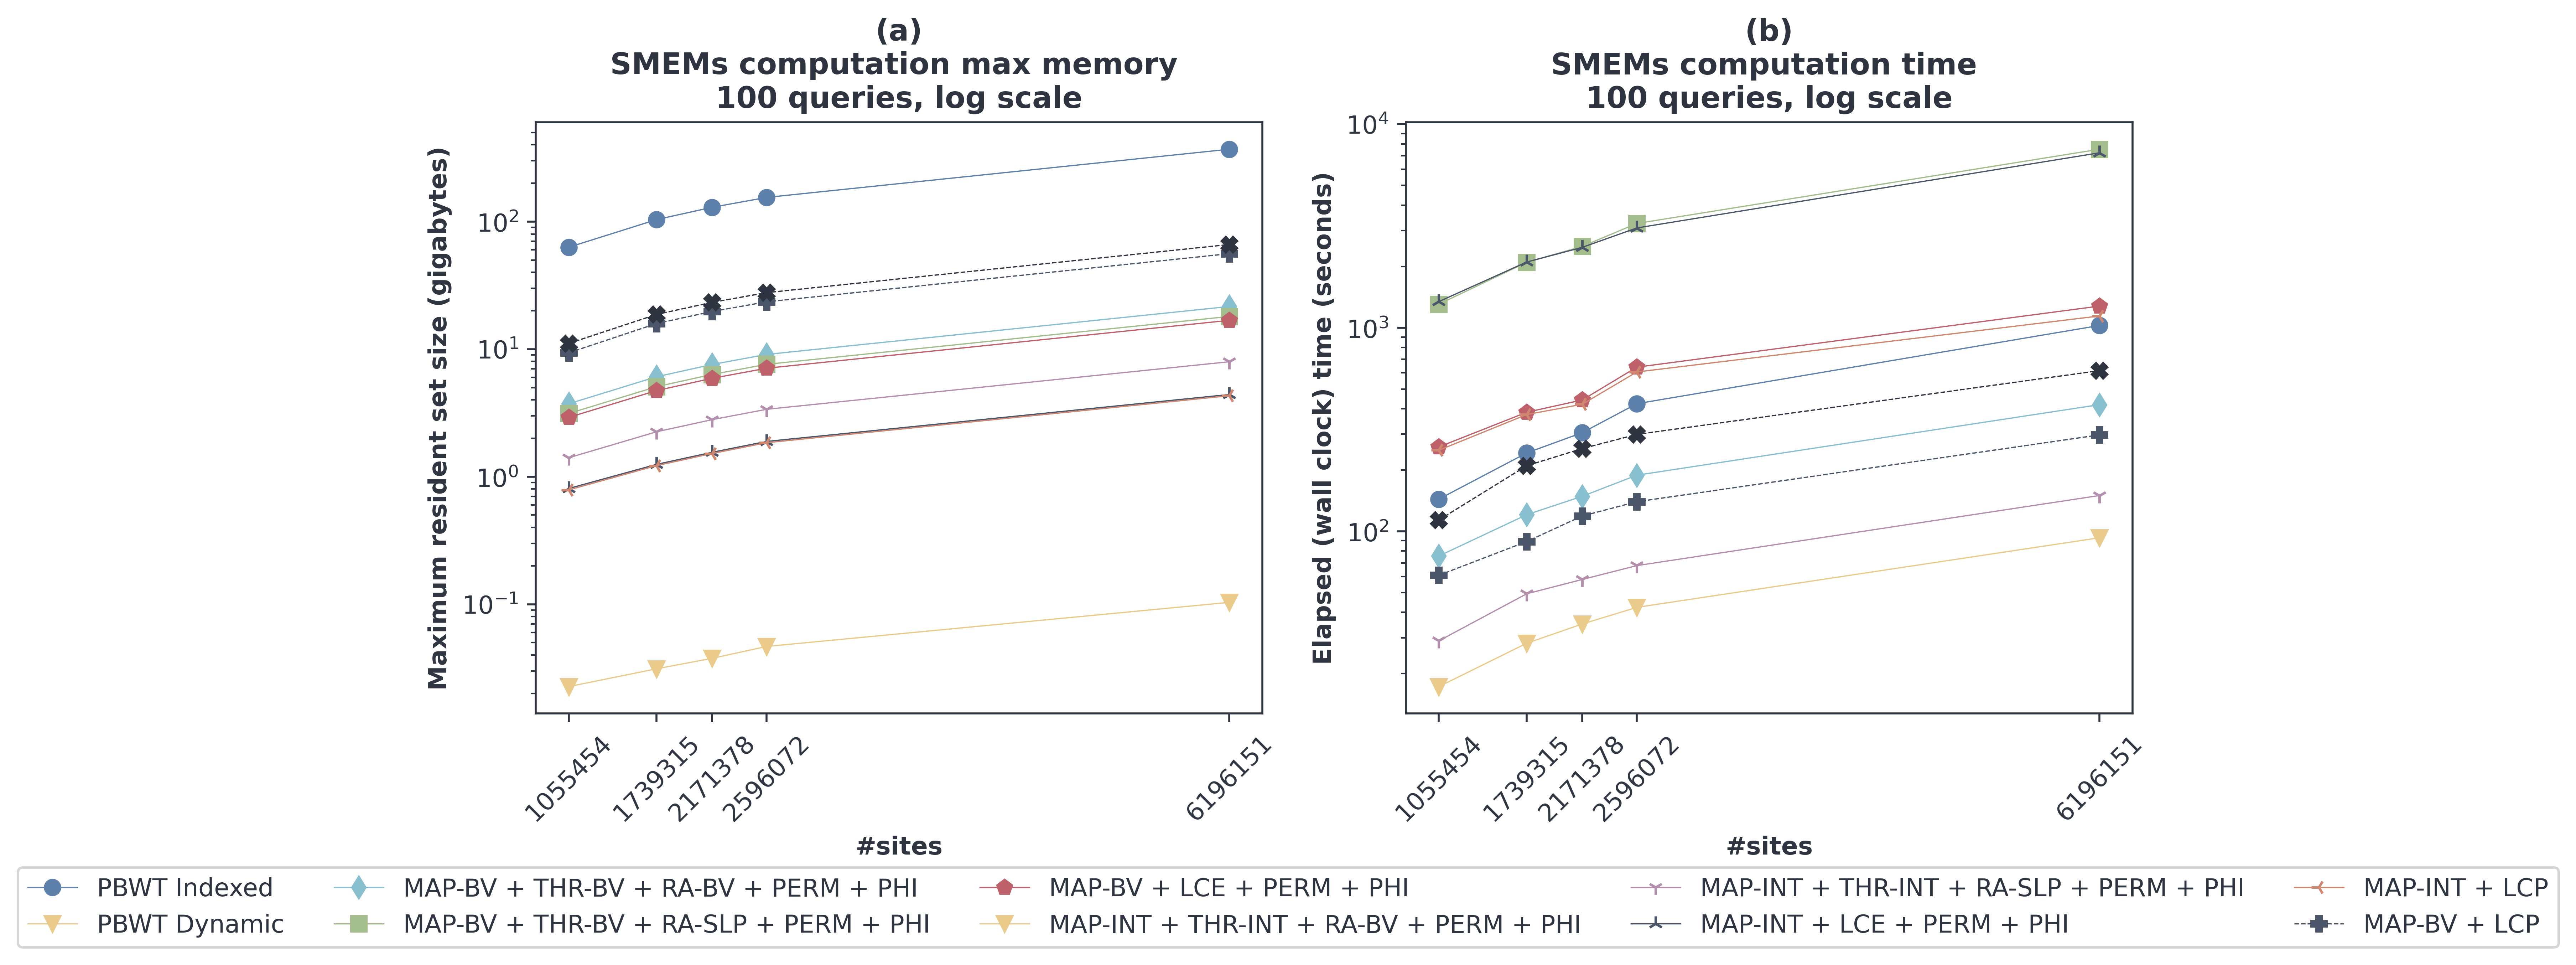
\includegraphics[width=\linewidth]{img/exe_time_mem_paper}
  \caption{Picchi di memoria (a) e tempi di esecuzione (b) per il calcolo degli
    SMEM.}
  \label{fig:smemtimememchr}
\end{figure}


\begin{table}
  \centering
  \caption{Risultati quantitativi dei picchi di memoria (gigabytes) di costruzione delle
    strutture dati.} 
  \label{tab:exemem}
  \footnotesize
  \subcaption*{\footnotesize{Tabella A: risultati relativi alla \textit{PBWT} e
      alle varianti 
    basate su \texttt{LCP} per la \textit{RLPBWT}.}} 
  \begin{tabular}{c||c|c|c|c} 
    \textbf{Chr}
    & \textbf{\texttt{matchIndexed}}
    & \textbf{\texttt{matchDynamic}}
    & \textbf{\texttt{MAP-INT \newline+ LCP}}
    & \textbf{\texttt{MAP-BV \newline+ LCP}}\\
    \hline
    \hline
    chr22 & 63 & 0.02 & 9 & 11 \\
    chr20 & 104 & 0.03 & 16 & 19 \\
    chr18 & 129 & 0.04 & 20 & 23 \\
    chr16 & 155 & 0.05 & 24 & 28 \\
    chr1 & 369 & 0.1 & 56 & 66 
  \end{tabular}
  \vspace{+3mm}
  \subcaption*{\footnotesize{Tabella B: risultati relativi alle varianti basate
      su 
      \textit{matching statistics} e \textit{bitvector sparsi} per la
      \textit{RLPBWT}.}}
  \vspace{+1mm}
  \begin{tabular}{c||c|c|c} 
    \textbf{Chr}
    & \textbf{\texttt{MAP/THR-BV + RA-BV $\cdots$}}
    & \textbf{\texttt{MAP/THR-BV + RA-SLP $\cdots$}}
    & \textbf{\texttt{MAP-BV + LCE $\cdots$}}\\
    \hline
    \hline
    chr22 & 4 & 3 & 3  \\
    chr20 & 6 & 5 & 5 \\
    chr18 & 8 & 6 & 6 \\
    chr16 & 9 & 8 & 7 \\
    chr1 & 22 & 18 & 17 
  \end{tabular}
  \vspace{+3mm}
  \subcaption*{\footnotesize{Tabella C: risultati relativi alle varianti basate
      su 
    \textit{matching statistics} e \textit{int vector compressi} per la
    \textit{RLPBWT}.}}
  \vspace{+1mm}
  \begin{tabular}{c||c|c|c} 
    \textbf{Chr}
    & \textbf{\texttt{MAP/THR-INT + RA-BV $\cdots$}}
    & \textbf{\texttt{MAP/THR-INT + RA-SLP $\cdots$}}
    & \textbf{\texttt{MAP-INT + LCE $\cdots$}}\\
    \hline
    \hline

    chr22 & 1,4 & 0,8 & 0,8 \\
    chr20 & 2,2 & 1,2 & 1,2 \\
    chr18 & 2,8 & 1,6 & 1,5 \\
    chr16 & 3,4 & 1,9 & 1,8 \\
    chr1 & 8,0 & 4,4 & 4,3 

                                                                        
  \end{tabular}
\end{table}


 

\begin{table}
  \centering
  \caption{Risultati quantitativi dei tempi (secondi) di calcolo degli
    \textit{SMEM}.}  
  \label{tab:exetime}
  \footnotesize
  \subcaption*{\footnotesize{Tabella A: risultati relativi alla \textit{PBWT} e
      alle varianti 
    basate su \texttt{LCP} per la \textit{RLPBWT}.}} 
  \begin{tabular}{c||c|c|c|c} 
    \textbf{Chr}
    & \textbf{\texttt{matchIndexed}}
    & \textbf{\texttt{matchDynamic}}
    & \textbf{\texttt{MAP-INT \newline+ LCP}}
    & \textbf{\texttt{MAP-BV \newline+ LCP}}\\
    \hline
    \hline
    chr22 & 144 & 17 & 61 & 114 \\
    chr20 & 243 & 28 & 89 & 210 \\
    chr18 & 305 & 35 & 119 & 255 \\
    chr16 & 424 & 42 & 140 & 299 \\
    chr1 & 1026 & 93 & 298 & 616
  \end{tabular}
  \vspace{+3mm}
  \subcaption*{\footnotesize{Tabella B: risultati relativi alle varianti basate
      su 
      \textit{matching statistics} e \textit{bitvector sparsi} per la
      \textit{RLPBWT}.}}
  \vspace{+1mm}
  \begin{tabular}{c||c|c|c} 
    \textbf{Chr}
    & \textbf{\texttt{MAP/THR-BV + RA-BV $\cdots$}}
    & \textbf{\texttt{MAP/THR-BV + RA-SLP $\cdots$}}
    & \textbf{\texttt{MAP-BV + LCE $\cdots$}}\\
    \hline
    \hline
    chr22 & 76 & 1305 & 260 \\
    chr20 & 121 & 2097 & 385  \\
    chr18 & 149 & 2509 & 442  \\
    chr16 & 189 & 3252 & 640 \\
    chr1 & 419 & 7531 & 1278 
  \end{tabular}
  \vspace{+3mm}
  \subcaption*{\footnotesize{Tabella C: risultati relativi alle varianti basate
      su 
    \textit{matching statistics} e \textit{int vector compressi} per la
    \textit{RLPBWT}.}}
  \vspace{+1mm}
  \begin{tabular}{c||c|c|c} 
    \textbf{Chr}
    & \textbf{\texttt{MAP/THR-INT + RA-BV $\cdots$}}
    & \textbf{\texttt{MAP/THR-INT + RA-SLP $\cdots$}}
    & \textbf{\texttt{MAP-INT + LCE $\cdots$}}\\
    \hline
    \hline
    chr22 & 29 & 1344 & 250 \\
    chr20 & 49 & 2103 & 375 \\
    chr18 & 58 & 2483 & 421 \\
    chr16 & 68 & 3092 & 606 \\
    chr1 & 150 & 7234 & 1142

  \end{tabular}
\end{table}
\dc{Controllare tutti questi dati}

\subsection{Tempo di una singola query}
Infine, per completare lo studio delle prestazioni temporali, si è deciso di
isolare il calcolo degli SMEM con ogni singola query, valutando media e
deviazione standard delle 100 query. A tal fine la misurazione è stata
effettuata sfruttando la libreria \texttt{time.h} presente nello standard del
linguaggio C, al fine di avere le medesime misurazioni sia con la \textit{PBWT}
che con la \textit{RLPBWT}. La misurazione è stata estremamente circoscritta, al
fine di misurare unicamente le istruzioni atte a cercare gli \textit{SMEM},
escludendo quelle per il computo degli indici o del caricamento delle strutture
dati.
Si segnala che nel caso dell'algoritmo \texttt{mathcDynamic} non si è
potuto, per natura stessa dell'algoritmo, isolare il computo degli indici
all'avanzamento alla colonna successiva. Resta esclusa, in ogni caso, la
costruzione della struttura base della \textit{PBWT}.
\dc{Non se dire questa cosa}
\\
Tale risultato è visualizzabile in figura
\ref{fig:smemsinglechr}, dove si è deciso di escludere le strutture
\texttt{MAP-INT + LCP} e \texttt{MAP-BV + LCP} in quanto non in grado di
computare quali righe presentino un certo \textit{SMEM}. I risultati
quantitativi sono consultabili in tabella \ref{tab:exetimesingle}. Anche in
questo caso, 
si conferma molto di quanto ipotizzato e discusso precedentemente. Caso a parte
è dato dall'algoritmo \texttt{matchDynamic}, che risulta avere le performance
peggiori, impiegando fino a cento volte il tempo dell\textit{'algoritmo 5} di
Durbin, ovvero \texttt{matchIndexed}. Per natura stessa dell'algoritmo, 
le operazioni sono studiate al fine di essere ottimizzate per pannelli di query
e non per una query singola. Nel caso in analisi, infatti, si hanno molte
operazioni che potrebbero essere ottimizzate per il caso della singola
query, caso invece dell'algoritmo \texttt{matchIndexed}. Sperimentalmente si è
quindi notato che una query o un centinaio di query hanno quindi all'incirca lo
tempo di calcolo. Infatti, prendendo ad esempio il cromosoma 1 si ha che tale
algoritmo impiega 93s per il calcolo con 100 query e una media di circa 88s (con
una deviazione standard di ben 7s) per
una singola query. Per quanto riguarda la \textit{RLPBWT}, con l'uso della
componente \texttt{RA-SLP}, si rilevano gli stessi problemi relativi all'random
access, precedentemente descritti. Questi problemi sono risolti con l'uso della
componente \texttt{RA-BV}. Inoltre, a parità di componenti per il mapping (e
conseguenti componenti per le threshold), l'uso della componente \texttt{LCE}
risulta più lenta dell'uso della componente \texttt{RA-BV}, a causa dei costi di
calcolo delle \textit{LCE query} stesse. Tutti questi sono risultati coerenti
con quanto visto nel caso di 100 query, anche in termini di migliori strutture
composte parlando di \textit{RLPBWT}. Si segnala che, oltre al fatto che non
sono qui misurate le tempistiche di caricamento delle strutture, le acquisizioni
dei dati 
per la singola query sono state ottenute in un momento diverso da quelle per 100
query, avendo, di conseguenza, una non perfetta proporzione tra i risultati.
\begin{figure}
  \centering
  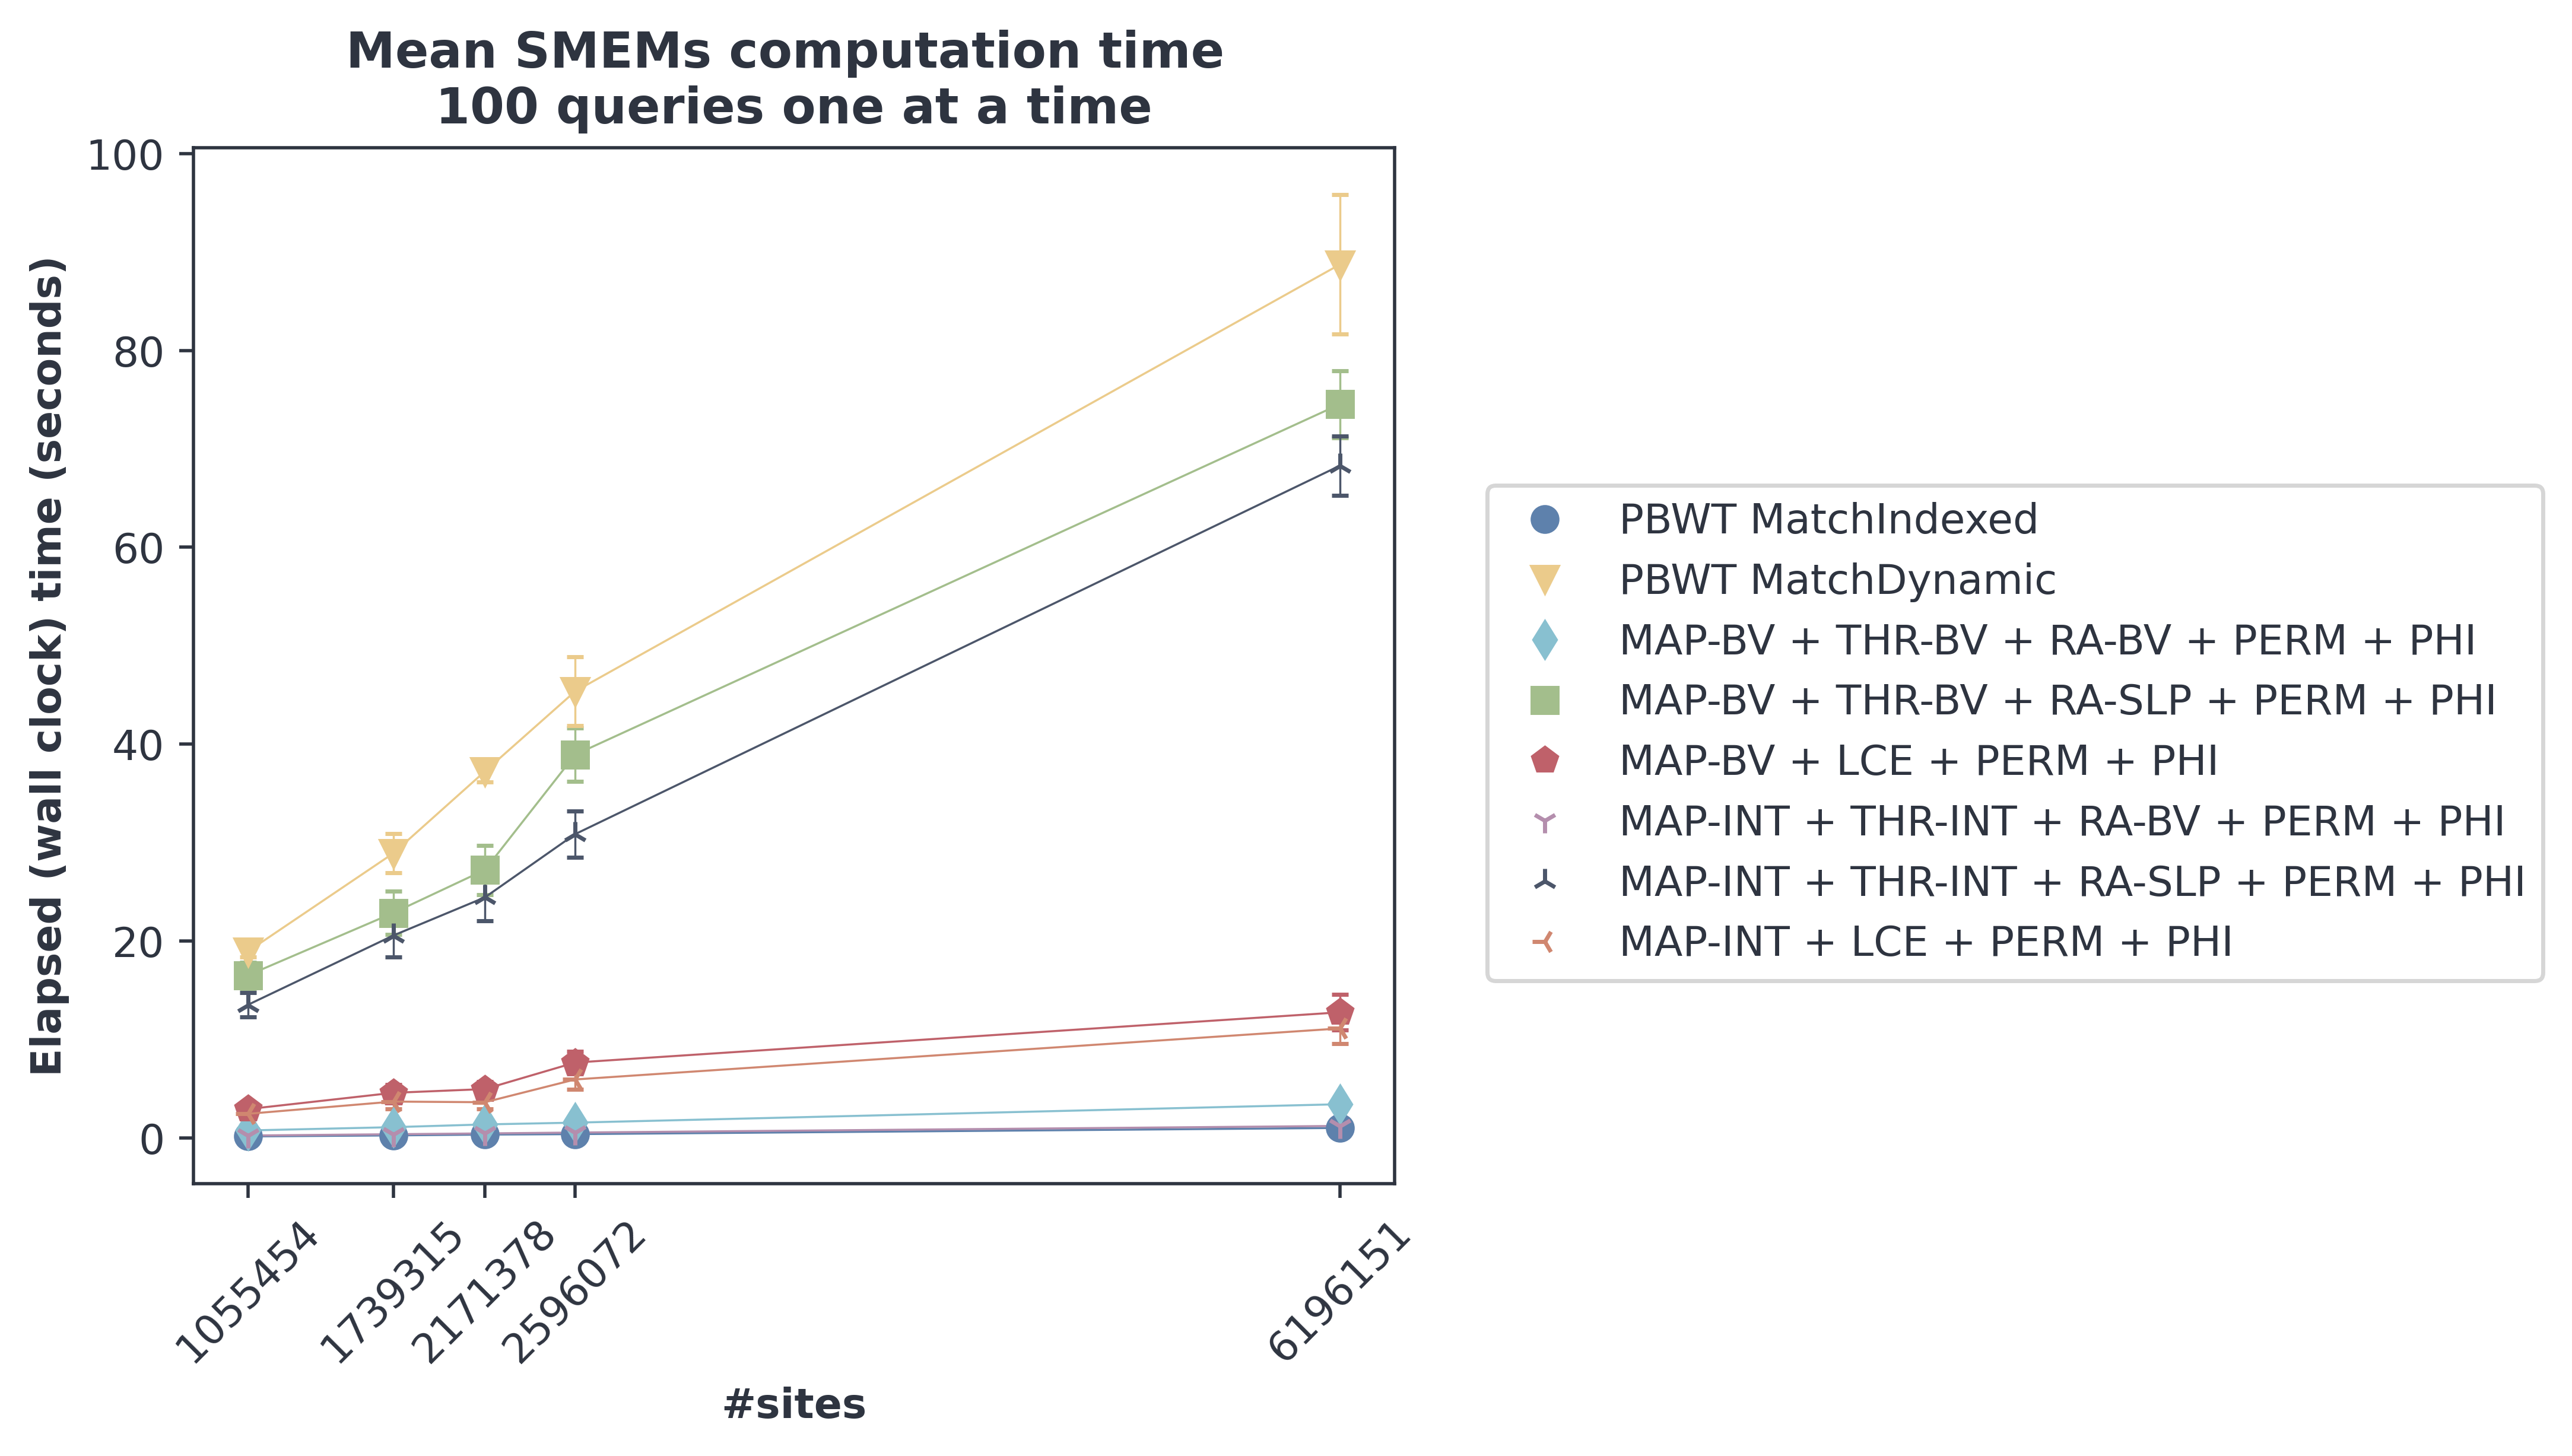
\includegraphics[width=\textwidth]{img/exe_time_single_paper.png}
  \caption{Tempo medio di esecuzione del calcolo degli SMEM per una singola
    query. Il grafico di destra è in scala logaritmica e, in entrambi, le
    barre d'errore rappresentano la deviazione standard.}
  \label{fig:smemsinglechr}
\end{figure}

\begin{table}
  \centering
  \caption{Risultati quantitativi dei tempi (secondi) di calcolo degli
    \textit{SMEM} su singola query. I risultati sono nella forma ``media $\pm$
    deviazione standard''.}  
  \label{tab:exetimesingle}
  \footnotesize
  \subcaption*{\footnotesize{Tabella A: risultati relativi alla \textit{PBWT}.}} 
  \begin{tabular}{c||c|c} 
    \textbf{Chr}
    & \textbf{\texttt{matchIndexed}}
    & \textbf{\texttt{matchDynamic}}\\
    \hline
    \hline
    chr22 & 0,15 $\pm$ 0,01 & 18,94 $\pm$ 0,58 \\
    chr20 & 0,25 $\pm$ 0,01 & 28,9 $\pm$ 1,99 \\
    chr18 & 0,33 $\pm$ 0,02 & 37,24 $\pm$ 1,08  \\
    chr16 & 0,38 $\pm$ 0,01 & 45,37 $\pm$ 3,49 \\
    chr1 & 1,01 $\pm$ 0,10 & 88,73 $\pm$ 7,08
  \end{tabular}
  \vspace{+3mm}
  \subcaption*{\footnotesize{Tabella B: risultati relativi alle varianti basate
      su 
      \textit{matching statistics} e \textit{bitvector sparsi} per la
      \textit{RLPBWT}.}}
  \vspace{+1mm}
  \begin{tabular}{c||c|c|c} 
    \textbf{Chr}
    & \textbf{\texttt{MAP/THR-BV + RA-BV $\cdots$}}
    & \textbf{\texttt{MAP/THR-BV + RA-SLP $\cdots$}}
    & \textbf{\texttt{MAP-BV + LCE $\cdots$}}\\
    \hline
    \hline
    chr22 & 0,75 $\pm$ 0,28 & 16,51 $\pm$ 1,34 & 2,92 $\pm$ 0,55\\
    chr20 & 1,08 $\pm$ 0,05 & 22,85 $\pm$ 2,21 & 4,57 $\pm$ 0,82\\
    chr18 & 1,36 $\pm$ 0,05 & 27,23 $\pm$ 2,50 & 4,96 $\pm$ 0,74 \\
    chr16 & 1,54 $\pm$ 0,05 & 38,93 $\pm$ 2,70 & 7,65 $\pm$ 1,14 \\
    chr1 & 3,41 $\pm$ 0,07 & 74,54 $\pm$ 3,40 & 12,75 $\pm$ 1,82 
  \end{tabular}
  \vspace{+3mm}
  \subcaption*{\footnotesize{Tabella C: risultati relativi alle varianti basate
      su 
    \textit{matching statistics} e \textit{int vector compressi} per la
    \textit{RLPBWT}.}}
  \vspace{+1mm}
  \begin{tabular}{c||c|c|c} 
    \textbf{Chr}
    & \textbf{\texttt{MAP/THR-INT + RA-BV $\cdots$}}
    & \textbf{\texttt{MAP/THR-INT + RA-SLP $\cdots$}}
    & \textbf{\texttt{MAP-INT + LCE $\cdots$}}\\
    \hline
    \hline
    chr22 & 0,24 $\pm$ 0,02 & 13,52 $\pm$ 1,26 & 2,44 $\pm$ 0,54 \\
    chr20 & 0,37 $\pm$ 0,03 & 20,55 $\pm$ 2,16 & 3,68 $\pm$ 0,74 \\
    chr18 & 0,45 $\pm$ 0,03 & 24,43 $\pm$ 2,38 & 3,62 $\pm$ 0,70 \\
    chr16 & 0,54 $\pm$ 0,03 & 30,86 $\pm$ 2,35 & 5,93 $\pm$ 1,01 \\
    chr1 & 1,21 $\pm$ 0,06 & 68,22 $\pm$ 3,02 & 11,12 $\pm$ 1,52

  \end{tabular}
\end{table}

% LocalWords:  sottostrutture
